\section{原子的位形: 卢瑟福模型}
\subsection{汤姆孙(Thomson)模型与卢瑟福(Rutherford)模型}
\begin{itemize}
\item \textbf{汤姆孙模型: }正电荷与负电荷均匀分布. (枣糕模型)
\item \textbf{卢瑟福模型: }正电荷集中于中心极小的区域,而等电荷的电子分布于中心以外的广大区域(核式模型). 
\end{itemize}

\subsection{库仑散射公式及推导}
\begin{itemize}
\item \textbf{公式}: 瞄准距离$b$为
\[
b=\frac{1}{2}\frac{1}{4\pi
\varepsilon_0}\frac{Z_1Z_2e^2}{E}\cot\frac{\theta}{2}
\]
\item \textbf{推导}: 由$F=ma$可得
\[
\frac{Z_1Z_2e^2}{4\pi\varepsilon_0r^2}\hat{r}=m\frac{\textrm{d}v}{dt}
\]
又因为库仑力作用线通过$Z_2$ ,因此库仑力对$Z_1$关于$Z_2$点的力矩为0,满足角动量守恒,即
\[
mr^2\frac{\textrm{d}\phi}{\textrm{d}t}=L\textrm{常量}
\]
由以上两式,消去时间因子可得
\[
\textrm{d}v=\frac{Z_1Z_2e^2}{4\pi\varepsilon_0L}\textrm{d}\phi\hat{r}
\]
由能量守恒可知数值上有 $v_i=V_f$,令 $v_i=v_f=v$,并对上式积分有
\[
v\sin\frac{\theta}{2}=\frac{1}{4\pi\varepsilon_0}\frac{Z_1Z_2e^2}{L}\cos\frac{\theta}{2}=\frac{1}{4\pi\varepsilon_0}\frac{Z_1Z_2e^2}{mvb}\cos\frac{\theta}{2}
\]
由于$mv^2=2E$,于是
\[
b=\frac{1}{2}\frac{1}{4\pi\varepsilon_0}\frac{Z_1Z_2e^2}{E}\cot\frac{\theta}{2}
\]
\begin{figure}[!htb]
\centering
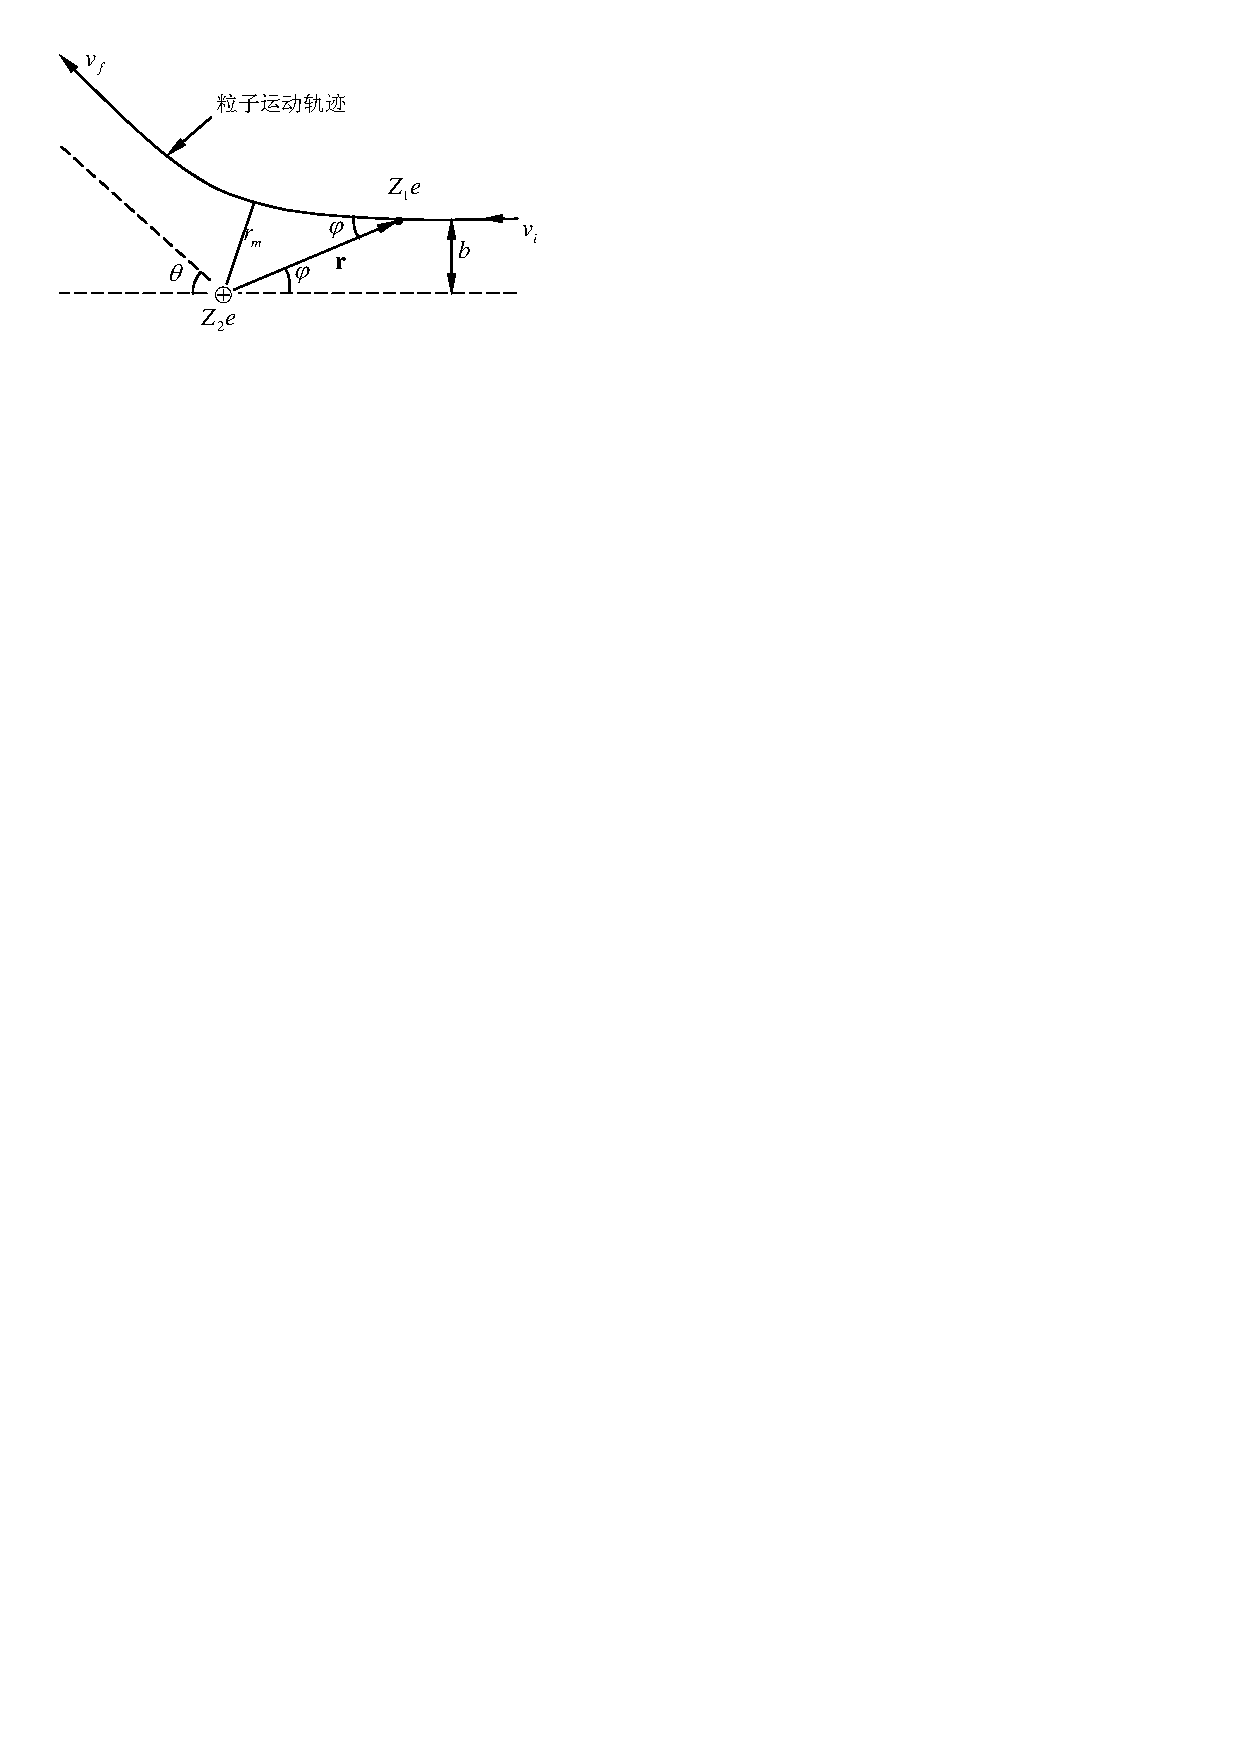
\includegraphics[width=0.5\textwidth]{fig01.pdf}
\caption{库仑散射}
\end{figure}
\end{itemize}

\subsection{卢瑟福公式及推导}
\begin{itemize}
\item \textbf{公式}: 微分截面$\sigma_c$为
\[
\sigma_c(\theta)=\Big(\frac{1}{4\pi\varepsilon_0}\frac{Z_1Z_2e^2}{4E}\Big)^2\frac{1}{\sin^2\frac{\theta}{2}}
\]
\item \textbf{推导}: 由库仑散射公式可知,瞄准距在$b$到$b+\textrm{d}b$之间的$\alpha$
粒子,经过散射必定向$\theta$到$\theta-\textrm{d}\theta$之间的角度射出. 设一薄箔的面积为$A$
,厚度为$t$(薄箔中的原子互相不遮蔽),环的面积为$2\pi
b|\textrm{d}b|$ ,则粒子打在这个环上的几率为
\[
\frac{2\pi
b|\textrm{d}b|}{A}=\frac{2\pi}{A}\Big(\frac{a}{2}\cot\frac{\theta}{2}\Big)
\Big|-\frac{a}{2}\csc^2\frac{\theta}{2}\cdot\frac{1}{2}\textrm{d}\theta\Big|
=\frac{a^22\pi
\sin\theta\textrm{d}\theta}{16A\sin^4\frac{\theta}{2}}
\]
由图\ref{fig02}可知,空心圆锥体的立体角与$\textrm{d}\theta$有: 
\[
\textrm{d}\Omega=\frac{2\pi r\sin\theta\cdot
r\text{d}\theta}{r^2}=2\pi \sin\theta\textrm{d}\theta
\]
由以上两式得
\[
\frac{2\pi
b|\textrm{d}b|}{A}=\frac{a^2\textrm{d}\Omega}{16A\sin^4\frac{\theta}{2}}
\]

一个薄箔有许多这样的圆环: 对应于一个原子核就有一个环;假如在单位体积内的原子核数为
$n$,则在体积$At$内共有$nAt$个环. 故被散射到$\theta$到
$\theta-\textrm{d}\theta$范围的几率为
\[
\textrm{d}p(\theta)=\frac{a^2\textrm{d}\Omega}{16A\sin^4\frac{\theta}{2}}nAt
\]
若有$N$个$\alpha$粒子打在薄箔上,则在$\textrm{d}\Omega$方向上测量到的$\alpha$
粒子数应为
\[
\textrm{d}N'=N\frac{a^2\textrm{d}\Omega}{16A\sin^4\frac{\theta}{2}}nAt
=ntN\Big(\frac{1}{4\pi\varepsilon_0}\frac{Z_1Z_2e^2}{4E}\Big)^2\frac{\textrm{d}\Omega}{\sin^4\frac{\theta}{2}}
\]
定义微分截面: 
\[
\sigma_c(\theta)=\Big(\frac{1}{4\pi\varepsilon_0}\frac{Z_1Z_2e^2}{4E}\Big)^2\frac{1}{\sin^2\frac{\theta}{2}}
\]

\begin{figure}[!htb]
\centering
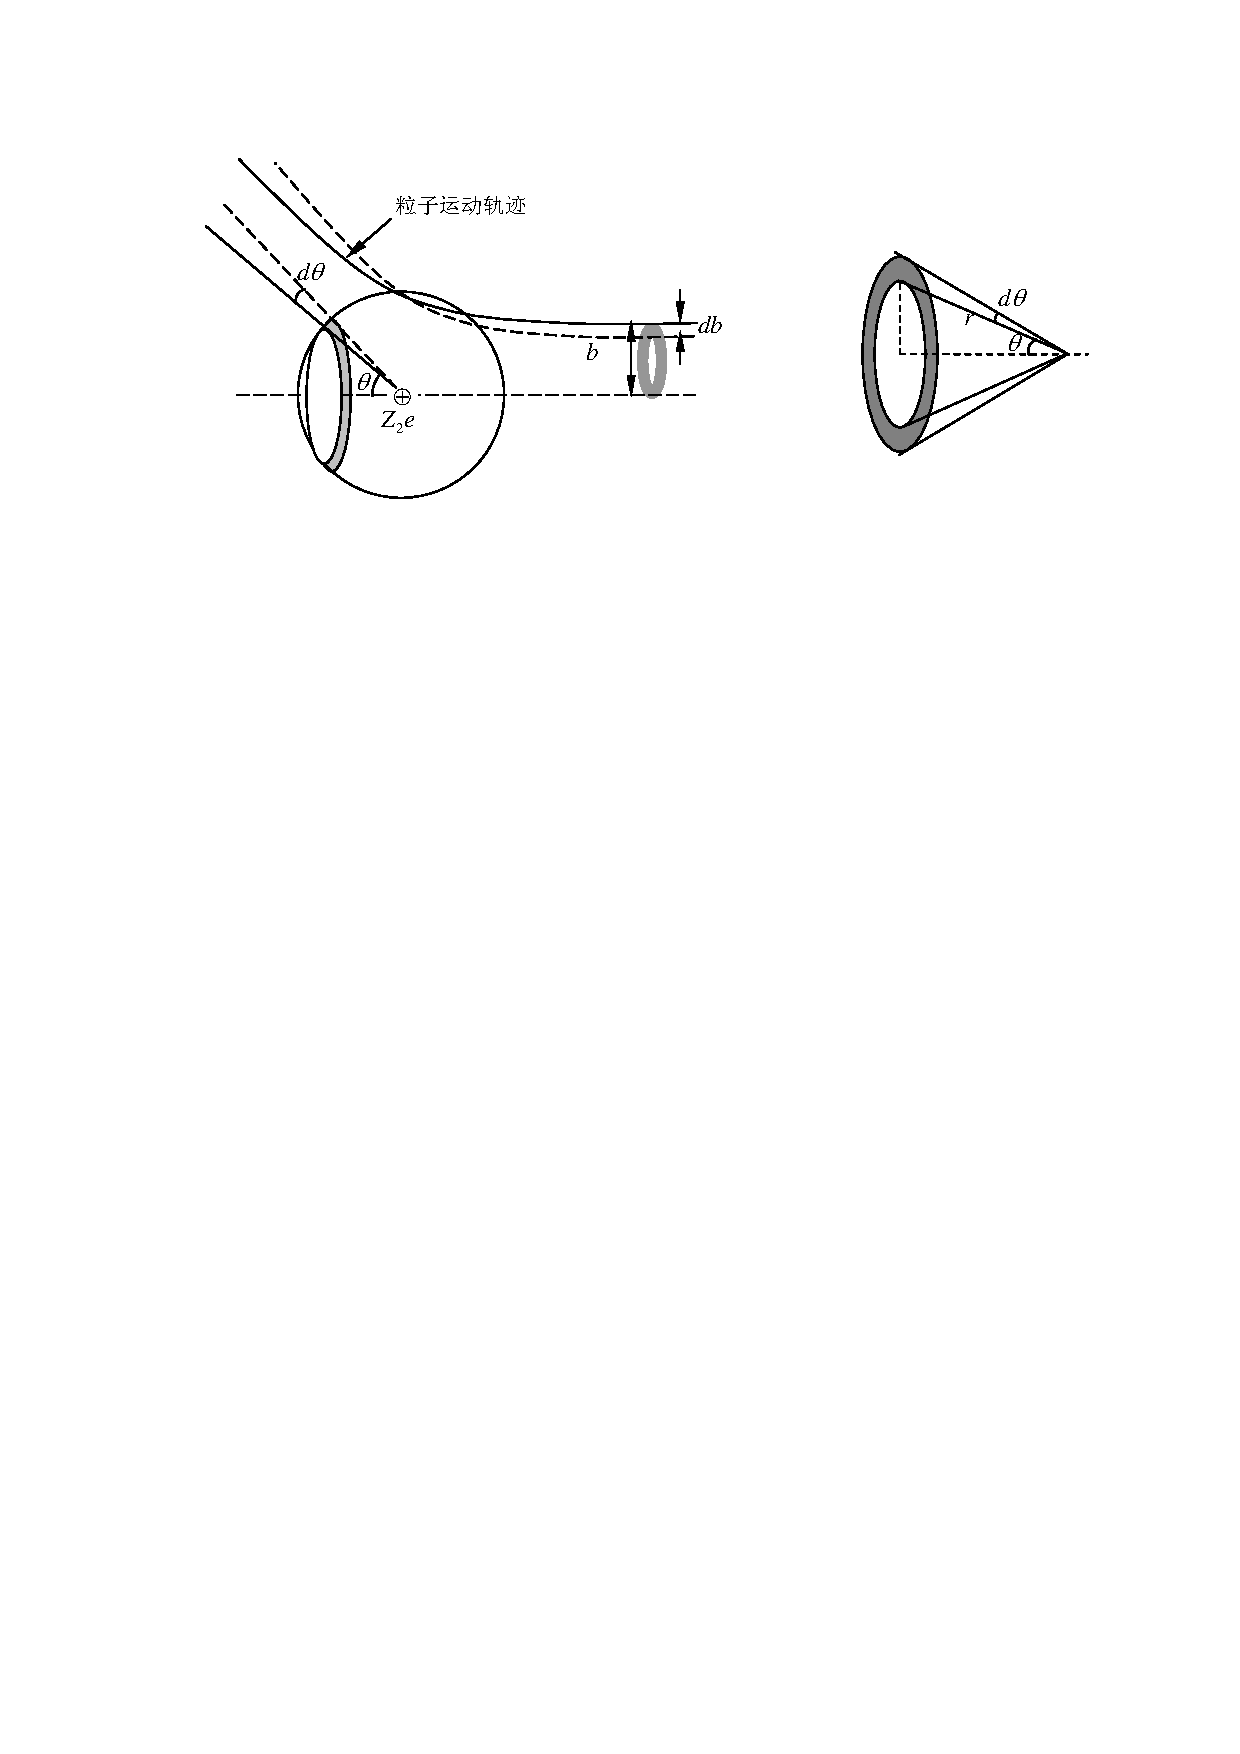
\includegraphics[width=0.7\textwidth]{fig02.pdf}
\caption{\label{fig02}卢瑟福公式}
\end{figure}
\item \textbf{意义}: $\sigma_c(\theta)$具有面积的量纲,它的物理意义是,$\alpha$粒子散射到$\theta$方向单位立体角内每个原子的有效散射截面. 
\end{itemize}

\subsection{行星模型的困难?}
\begin{multicols}{2} 
课本中有这样一段话(P25): ``谁都知道,任何带电粒子在作加速运动的过程中都要以发射电磁波方式放出能量. 这样, 电子就不能永远绕原子核转下去
. ''这句话对吗?

\begin{center}
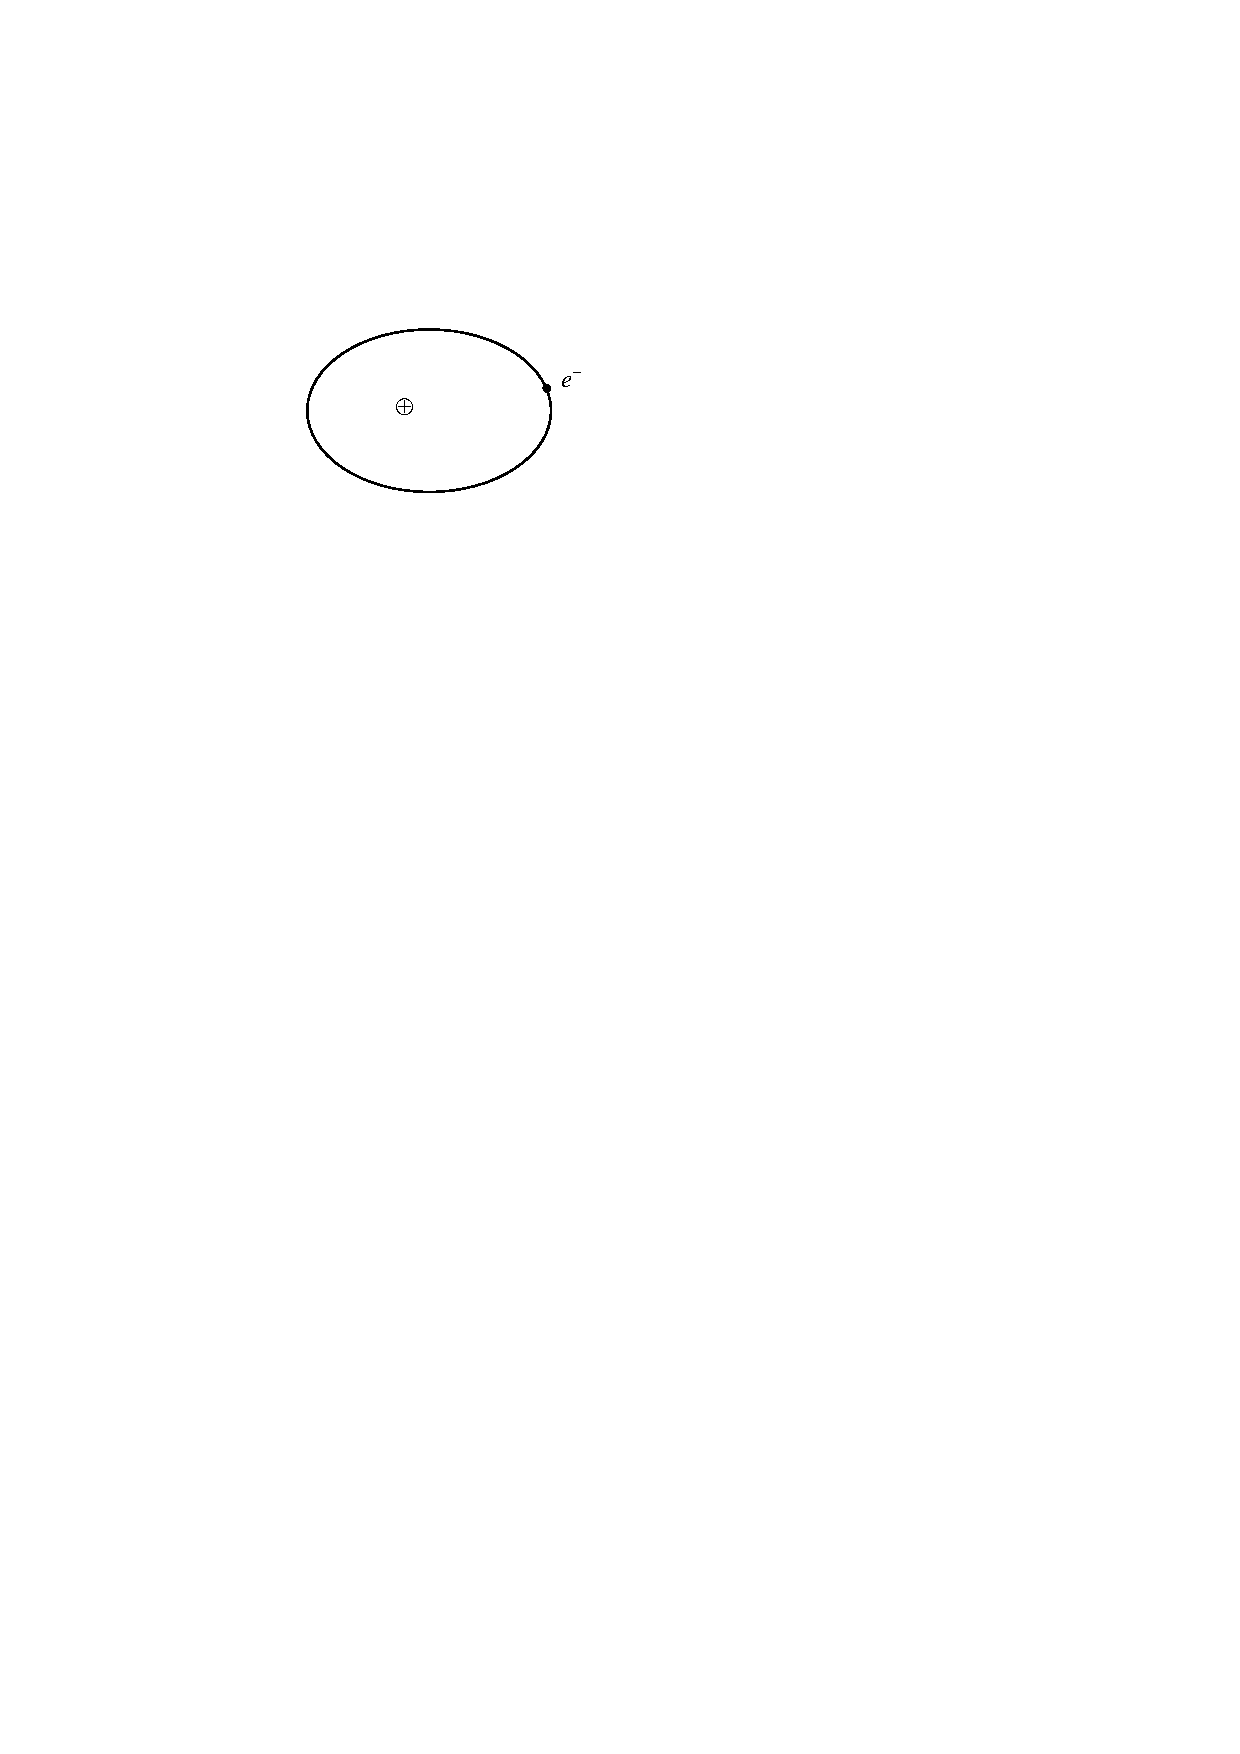
\includegraphics[width=0.175\textwidth]{fig15.pdf}
\end{center}
\end{multicols}

\vspace{-1em}
从经典力学出发,讨论行星模型电子到底能不能永远绕原子核转下去. 对原子系统,外力忽略不计,则有
\[
\textrm{没有能量交换}\Longrightarrow\frac{\textrm{d}E_{atom}}{\textrm{d}t}=0
\]
\[
\sum
\overrightarrow{r_{ic}}\times\overrightarrow{f_i^e}=\frac{\textrm{d}\sum\overrightarrow{r_{ic}}\times
m_i\dot{\overrightarrow{r_{ic}}} }{\textrm{d}t}=0
\quad \Longrightarrow\quad
\textrm{角动量}\sum\overrightarrow{r_{ic}}\times
m_{i}\dot{\overrightarrow{r_{ic}}}=\overrightarrow{C}\textrm{常矢量}
\]
结果与课本中的结论相反,这与我们所知道的: 地球绕了太阳几亿年也没落到太阳上一样. 
